% Thesis appendix item: ecfp4_overview
% Seeded on 2026-09-27 from qsar_qm_models/supplementary/items/ecfp4_overview.tex by thesis_appendix/seed_from_paper.py.
% From here on this copy is edited independently of the paper. Rules: thesis_appendix/README.md.
% The lines below, down to the first blank line, are the PAPER copy's header, kept for
% provenance. They describe the paper file, not this one: in particular a GENERATED
% notice there does not apply here, and this copy may be edited by hand.
% Supplementary item: ecfp4_overview
% Split out of additional_files.tex on 2026-09-27, where it was Additional file 6 (ECFP4 global overview (was Supp Figure S1)).
% Content unchanged apart from: the heading line removed (the build writes it), the old
% 'Table S*/Figure S*' caption prefix replaced by \SuppFile{}, and the label renamed to supp:ecfp4_overview.
% Rules: supplementary/README.md.

\begin{figure}[H]
\centering
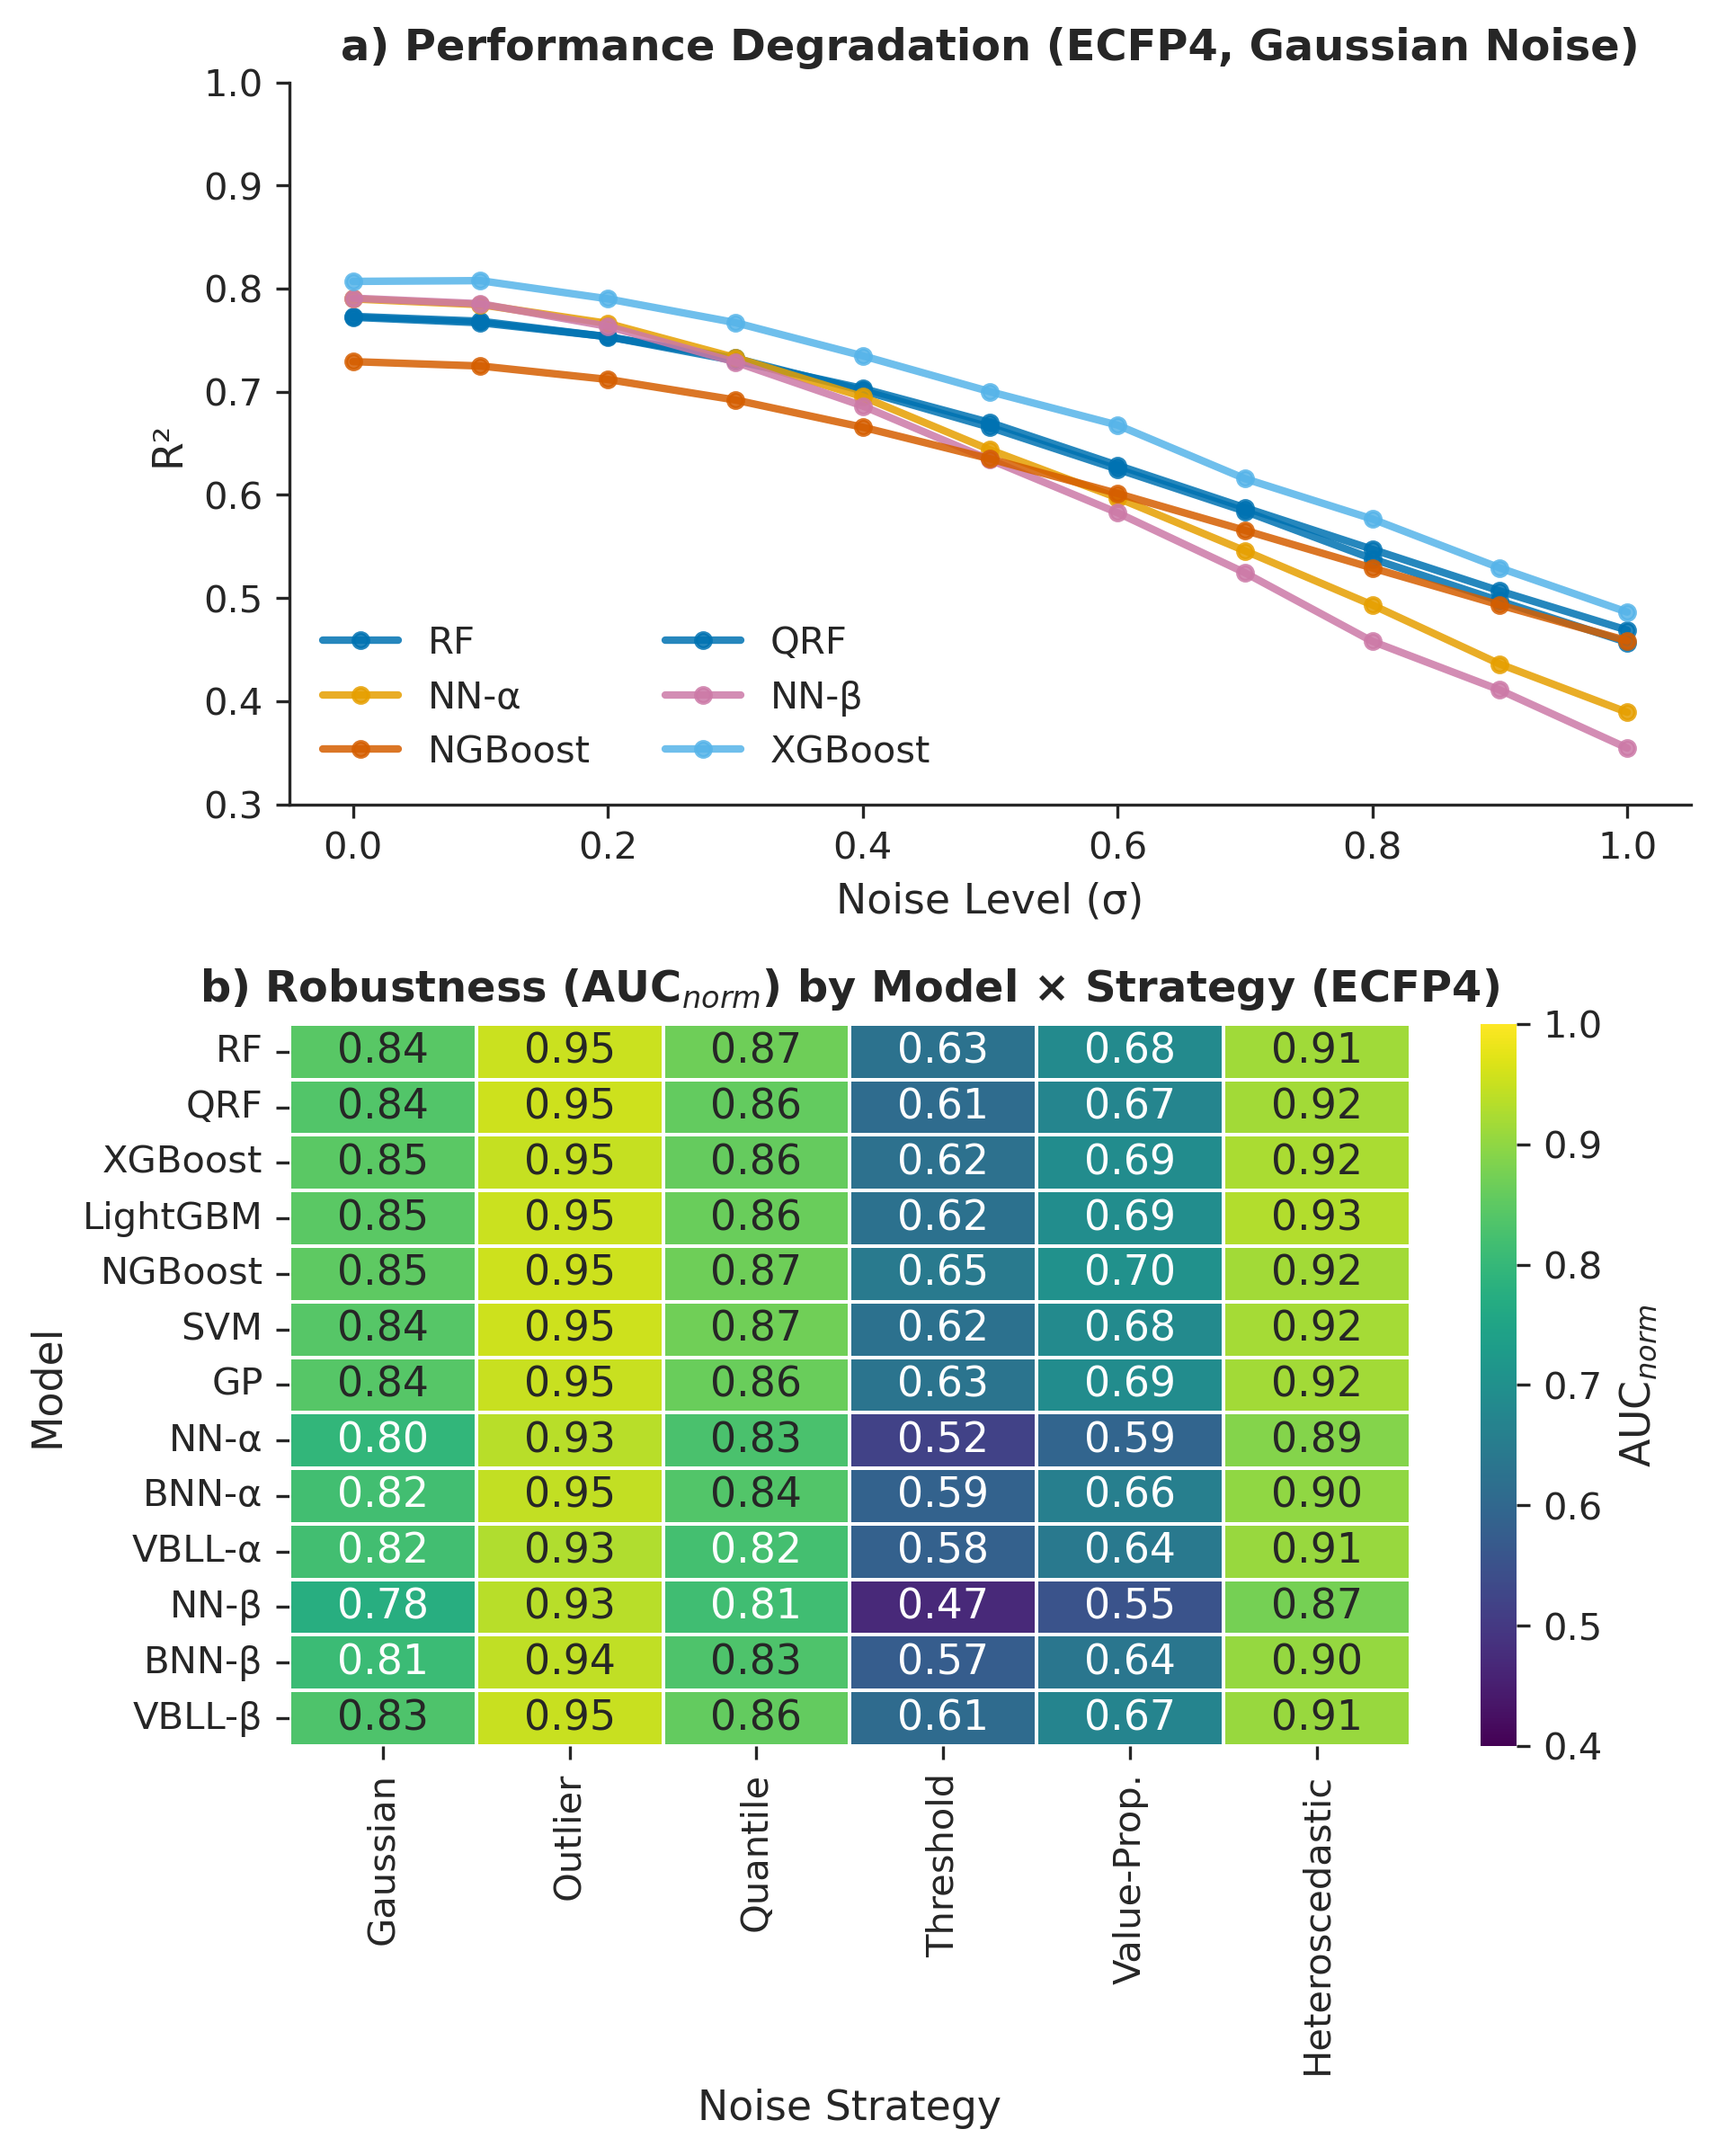
\includegraphics[width=\textwidth,height=0.78\textheight,keepaspectratio]{fig1_supp_ecfp4_overview.png}
\caption{\textbf{Global overview of noise robustness on the ECFP4 representation, evaluated on QM9 HOMO--LUMO gap.}
a) Performance degradation curves (R$^2$ versus noise level $\sigma$) under Gaussian noise. b) Noise degradation slope (NDS) heatmap across model architectures and noise strategies; lower (more negative) NDS indicates faster degradation under noise.}
\label{app:noise:ecfp4_overview}
\end{figure}
